\chapter{METODOLOGI}
% Ubah bagian-bagian berikut dengan isi dari desain dan implementasi

Eksperimen pada penelitian ini akan mengikuti konvensi standar eksperimen DRL sebelumnya, yaitu menguji coba dan mengevaluasi performa agen dalam \emph{environment} dengan membandingkan nilai \emph{reward} yang diterima oleh agen.
Agen akan melakukan \emph{training} dalam \emph{environment} yang telah dibuat.

\section{Perangkat}

Eksperimen dalam penelitian ini menggunakan beberapa perangkat keras dan perangkat lunak.


\subsection{Perangkat Keras}

Proses \emph{training} agen dilakukan dengan sebuah komputer. Komputer tersebut memiliki spesifikasi:
\begin{itemize}
  \item Processor: Intel I7 9700K
  \item Graphics Card: RTX 2080 SUPER
  \item RAM: 32GB DDR4
  \item SSD: 512GB NVME PCIE Gen 3
\end{itemize}

\subsection{Perangkat Lunak}

Beberapa pernagkat lunak digunakan untuk menunjang pembuatan \emph{environment} dan agen DRL dalam eksperimen ini:
\begin{itemize}
  \item Python
  \item Visual Studio Code
  \item Tensorboard
  \item Ray RLlib
  \item Pygame
  \item PettingZoo
  \item Numpy
  \item Matplotlib
\end{itemize}
\section{Desain Environment}
Desain dari \emph{environment} adalah modifikasi dari Inquisitive Otter's Civ6 environment \citep{civ6Environment}. 
Desain awal dari \emph{environment} ini hanya memiliki sebuah agen \emph{attacker} dan memiliki mekanisme yang kurang sesuai dengan mekanisme Civ6.
\emph{Environment} yang sudah dimodifikasi ini juga sudah diimplementasikan ke dalam PettingZoo.
Implementasi ke PettingZoo memudahkan untuk mengintegrasikan \emph{environment} ini dengan library RL lain.

\subsection{Area dan Posisi}
\emph{Environment} merupakan area \emph{pointy top hexagonal grid} berukuran 8x8. Di tengah area tersebut terdapat sebuah kota.
\emph{Environment} yang sudah termodifikasi memiliki dua jenis agen yaitu agen \emph{attacker} dan agen \emph{defender}.
Agen \emph{attacker} memiliki 3 \emph{unit} jarak dekat (\emph{melee}) (\emph{warrior}) dan 2 \emph{unit} jarak jauh (\emph{ranged}) (\emph{slinger}).
Agen \emph{defender} memiliki 2 \emph{warrior} dan 1 \emph{slinger}.

Penempatan \emph{unit} agen dilakukan secara acak dengan pembatasan.
\emph{Unit} agen \emph{attacker} ditempatkan minimal sejauh 5 lantai dari kota di tengah area.
\emph{Unit} agen \emph{defender} berada di lantai sebelah kota.


\begin{figure}[H]
  \centering
    % Nama dari file gambar yang diinputkan
    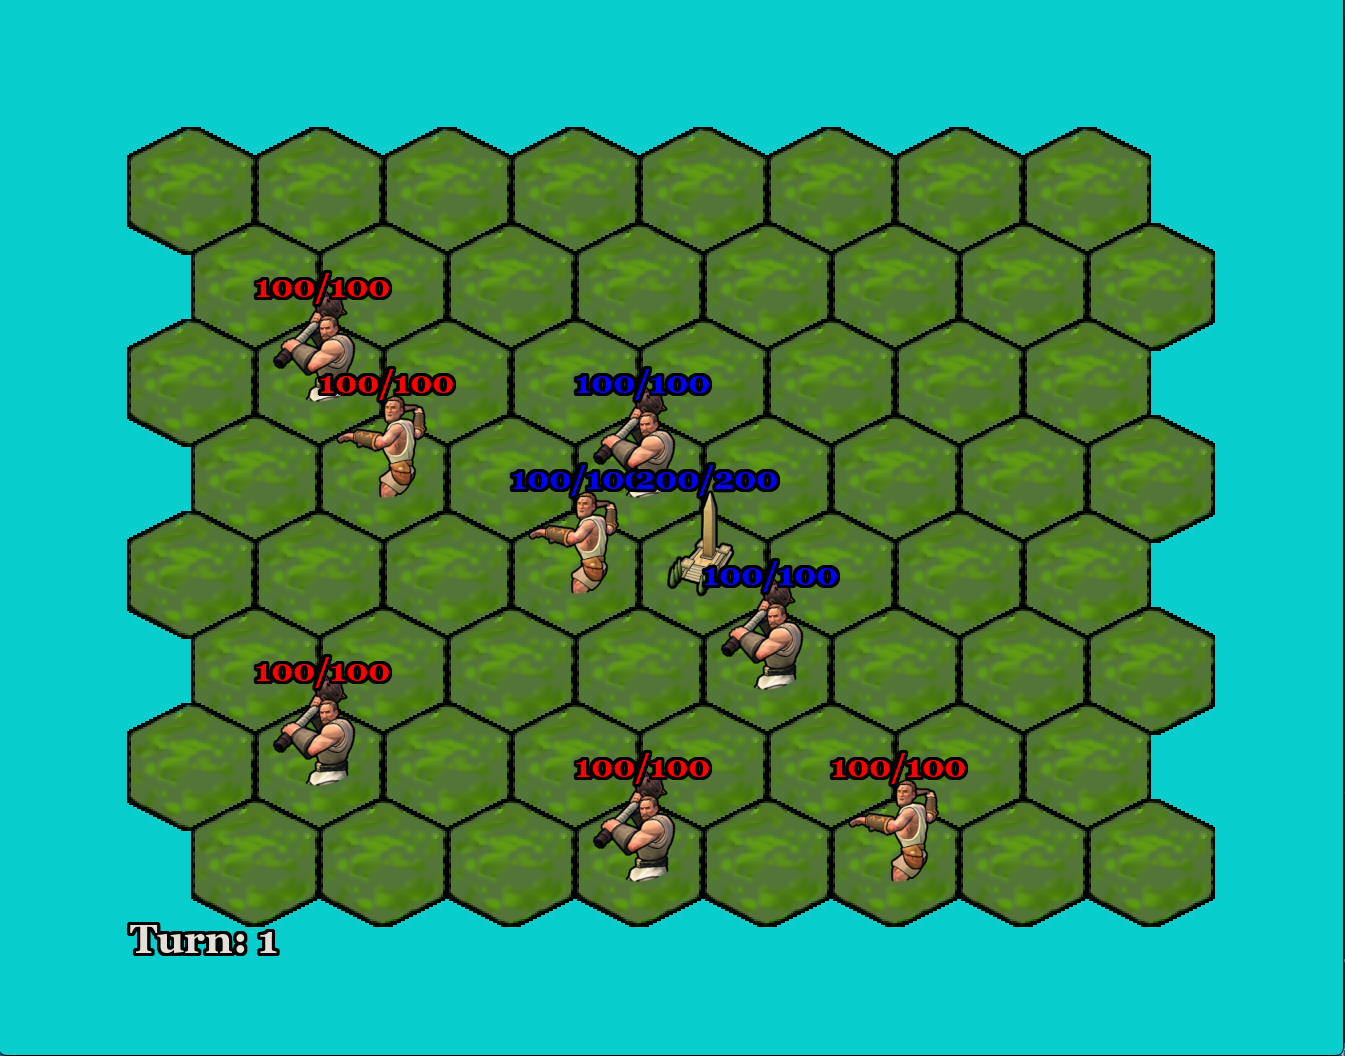
\includegraphics[scale=0.3]{gambar/environment_screenshot.png}
    % Keterangan gambar yang diinputkan
    \caption{\emph{Screenshot environment} dalam mode \emph{render}. \emph{Unit} milik agen \emph{attacker} memiliki teks \emph{hit points} berwarna merah dan unit milik agen \emph{defender} memiliki teks \emph{hit points} berwarna biru.}
    % Label referensi dari gambar yang diinputkan
    \label{fig:environmentScreenshot}
\end{figure}

\subsection{Unit dan Kota}
\emph{Unit} yang paling banyak jumlahnya dalam \emph{environment} ini adalah \emph{warrior}. 
\emph{Warrior} merupakan \emph{melee unit}, yang mana hanya dapat menyerang lawan yang berada di sebelah unit tersebut.
\emph{Warrior} memiliki attribut sebagai berikut:
\begin{itemize}
  \item HP: 100
  \item \emph{Movement Points}: 2
  \item \emph{Combat Strength}: 20
\end{itemize}

Jenis \emph{Unit} kedua adalah \emph{slinger}. \emph{Slinger} merupakan \emph{ranged unit} yang memiliki jarak sejauh 1 lantai.
\emph{Slinger} dapat menyerang \emph{unit} lain yang berdekatan dengan \emph{slinger} tanpa menerima \emph{damage} balasan dari \emph{unit} yang diserang.
\emph{Slinger} memiliki attribut sebagai berikut:
\begin{itemize}
  \item HP: 100
  \item \emph{Movement Points}: 2
  \item \emph{Combat Strength}: 5
  \item \emph{Ranged Strength}: 15
\end{itemize}

Kota merupakan tujuan utama yang perlu dihancurkan oleh agen \emph{attacker}. 
Kota akan berusaha melakukan perbaikan pada gilirannya dengan menambahkan +20 HP jika HP yang dimilikinya kurang dari nilai maksimum.
Kota tidak dapat melakukan perbaikan jika terdapat minimal tiga \emph{melee unit} milik agen \emph{attacker}.
Berikut adalah attribut dari kota:
\begin{itemize}
  \item HP: 200
  \item \emph{Combat Strength}: 28
\end{itemize}

\begin{figure}[!htb]
  \begin{minipage}{0.32\textwidth}
    \centering
    
\includegraphics[width=\linewidth]{gambar/warrior_1.png}
    \caption{\emph{Unit warrior}}\label{Fig:warrior}
  \end{minipage}\hfill
  \begin{minipage}{0.32\textwidth}
    \centering
    
\includegraphics[width=\linewidth]{gambar/slinger_1.png}
    \caption{\emph{Unit slinger}}\label{Fig:slinger}
  \end{minipage}
  \begin{minipage}{0.32\textwidth}
    \centering
    
\includegraphics[width=\linewidth]{gambar/city.png}
    \caption{Kota}\label{Fig:kota}
  \end{minipage}
\end{figure}

\subsection{Giliran dan Pergerakan Unit Agen}
Agen dapat mengkontrol \emph{unit} mereka pada giliran yang sudah ditentukan. 
\emph{Environment} dimulai dengan giliran agen \emph{attacker}, dilanjutkan oleh giliran kota, dan kemudian
ke giliran agen \emph{defender} sebelum kembali ke agen \emph{attacker}. 
Pergerakan dan pemilihan unit oleh agen dilakukan secara sekuensial. Pertama, agen akan memilih unit pertama mereka.
Agen akan melakukan pergerakan dengan unit yang telah dipilih sampai unit tersebut tidak lagi memiliki \emph{movement points}
pada giliran tersebut.
Setelah itu, agen akan berpindah ke unit selanjutnya. Hal ini akan berulang sampai agen tidak lagi memiliki unit yang masih
mempunyai \emph{movement points}. Jika agen sudah tidak memiliki unit yang masih mempunyai \emph{movement points}
maka agen akan mengakhiri giliran mereka dan giliran berikutnya akan dimulai. 
Sebuah \emph{episode} dari \emph{environment} akan berakhir ketika 20 giliran sudah berlalu, kota sudah hancur, atau seluruh \emph{unit}
milik agen \emph{attacker} mati.
Berikut flowchart dari pergerakan dan pemilihan sekuensial ini:

\begin{figure}[H]
  \centering
    % Nama dari file gambar yang diinputkan
    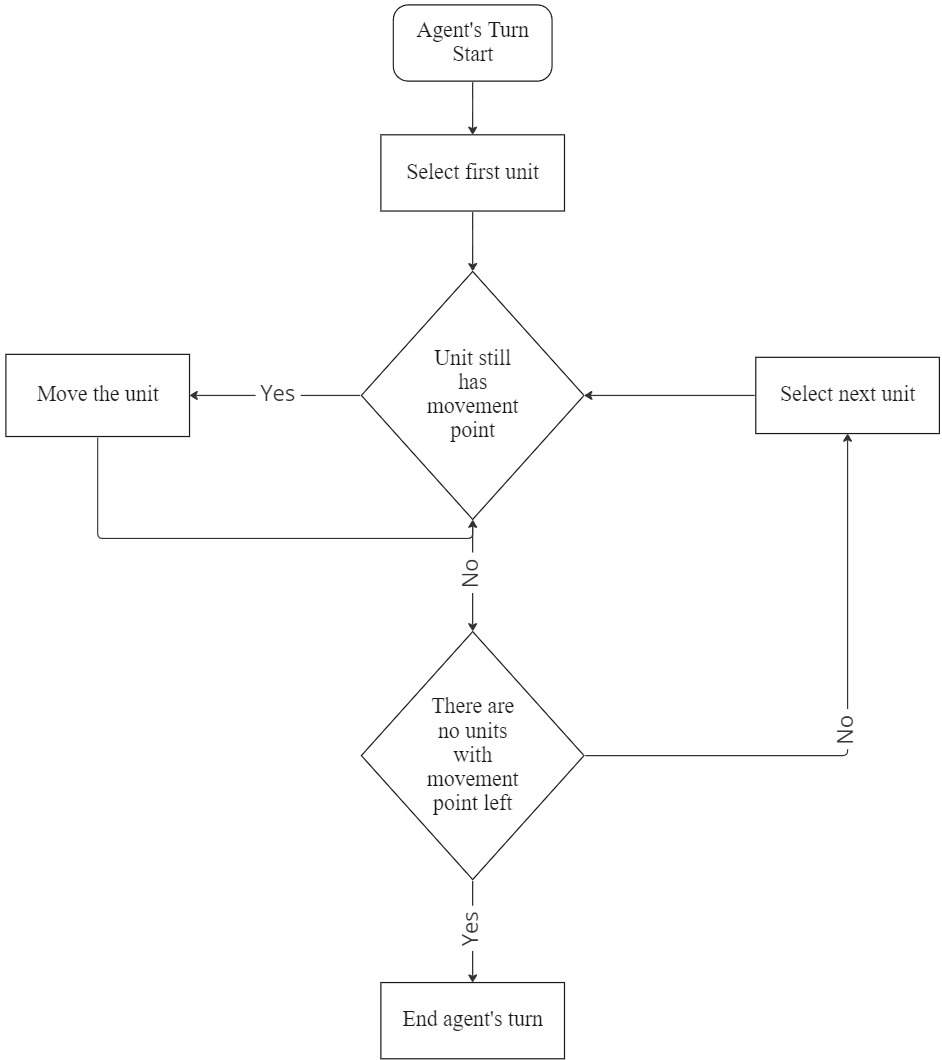
\includegraphics[scale=0.48]{gambar/unit_sequential_movement.jpg}
    % Keterangan gambar yang diinputkan
    \caption{\emph{Flowchart} pergerakan dan pemilihan sekuensial unit agen}
    % Label referensi dari gambar yang diinputkan
    \label{fig:sequentialMovementFlowchart}
\end{figure}

\subsection{Action Space}
\emph{Action space} merupakan kemungkinan yang dapat diambil oleh agen untuk melakukan sebuah \emph{action}.
\emph{Action space} yang digunakan dalam \emph{environment} ini adalah berupa 7 \emph{discrete actions}.
7 \emph{discrete actions} tersebut merupakan 6 sisi dimana unit dapat bergerak ke dan 1 \emph{action} unit tidak bergerak ke manapun.

% input gambar
\begin{figure}[H]
  \centering
    % Nama dari file gambar yang diinputkan
    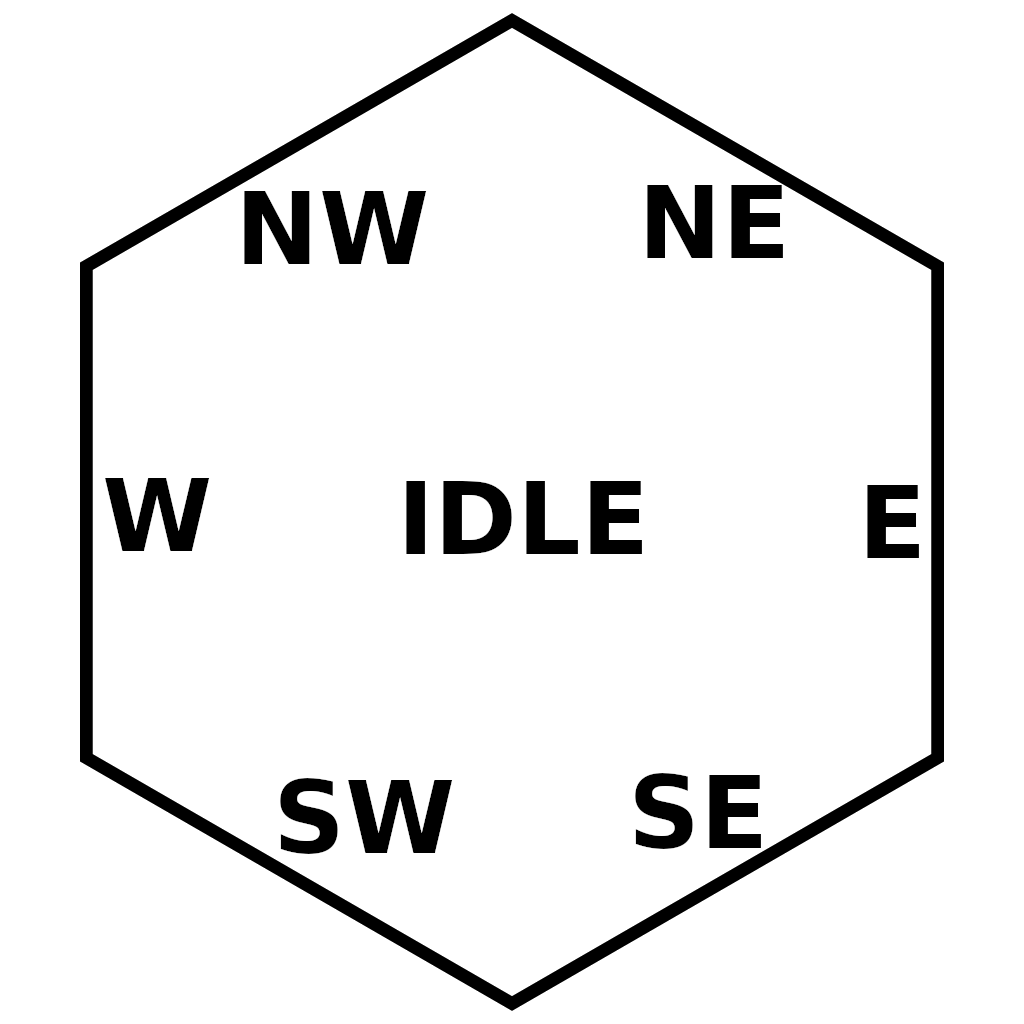
\includegraphics[scale=0.6]{gambar/hex_action.png}
    % Keterangan gambar yang diinputkan
    \caption{7 \emph{actions} yang dapat diambil oleh AI dalam \emph{Hexagonal tile}}
    % Label referensi dari gambar yang diinputkan
    \label{fig:hex_action}
\end{figure}

\subsection{Observation Space}
\emph{Observation Space} merupakan kumpulan \emph{state} dalam \emph{environment} yang didapatkan oleh agen saat melakukan observasi.
Agen dalam \emph{environment} penelitian ini melakukan \emph{complete observation}. 
Kedua agen mendapatkan informasi \emph{state} yang penuh dan sama saat melakukan observasi.
Seluruh nilai \emph{state} dinormalisasi sehingga nilainya berupa 0 sampai 1.
Berikut merupakan \emph{state} yang didapatkan oleh agen saat observasi:
\begin{itemize}
  \item Jarak seluruh unit dari kota: $x_{1}, y_{1}, \dots x_{n}, y_{n}$
  \item Nilai HP dari seluruh unit: $HP_{1}, \dots HP_{n}$
  \item Nilai movement points dari seluruh unit: $MP_{1}, \dots MP_{n}$
\end{itemize}

\subsection{Reward Agen}
\emph{Reward} merupakan nilai yang diberikan kepada agen ketika agen tersebut melakukan sebuah \emph{action}.
Karena \emph{environment} pada penelitian ini merupakan \emph{asymmetric}, maka terdapat dua tipe \emph{reward}:
\emph{general rewards} dan \emph{attacker rewards}. 
\emph{General rewards} adalah tipe \emph{reward} yang diberikan ke agen \emph{attacker} dan \emph{defender}.
Sedangkan \emph{attacker rewards} hanya diberikan pada agen \emph{attacker}.
Berikut \emph{reward} tersebut:
\begin{itemize}
  \item General rewards: \begin{itemize}
      \item Bergerak ke luar batas \emph{environment} = -1
      \item Melakukan \emph{healing} pada sebuah \emph{unit} = +0.1
      \item Menyerang \emph{unit} lawan = +0.2
      \item Mematikan \emph{unit} lawan = +3
  \end{itemize}
  \item Attacker rewards: \begin{itemize}
      \item Menghancurkan kota = +20
      \item Menyerang kota = +0.5
      \item Kota melakukan perbaikan = -0.3
      \item Sebuah \emph{unit} mati = -1
      \item Sebuah giliran telah berlalu = -1
  \end{itemize}
\end{itemize}

Agen \emph{attacker} akan mendapatkan +20 poin ketika menghancurkan kota, karena itu merupakan tujuan utama dari agen \emph{attacker}.
Jika sebuah \emph{unit} agen \emph{attacker} mati atau sebuah giliran telah berlalu maka agen \emph{attacker} akan mendapatkan -1 point
Hal ini untuk memaksa agen \emph{attacker} agar menyelesaikan tujuannya secepat mungkin dan meminimalisir kehilangan \emph{unit}.

Agen \emph{defender} yang memiliki tujuan untuk mencoba mencegah agen \emph{attacker} mendapatkan +3 poin ketika sebuah \emph{unit}
agen \emph{attacker} mati. Tidak diberikan penalti pada agen \emph{defender} ketika unit mereka mati karena pada eksperimen sebelumnya,
hal tersebut membuat agen \emph{defender} terlalu pasif. Kedua agen akan mendapatkan penalti ketika mencoba untuk menggerakan \emph{unit}
milik mereka keluar dari batas \emph{environment}.

\section{Implementasi Algoritma DRL}
Implementasi algoritma dalam penelitian ini menggunakan RLlib versi 2.0.0.
Kami menggunakan RLlib dengan alasan bahwa algoritma yang diimplementasikan dalam \emph{library} ini
sudah diverifikasi oleh berbagai pihak, sehingga menghindari adanya \emph{bug} pada implementasi manual.
Alasan kedua adalah kemampuan RLlib untuk diintegrasikan dengan simulator eksternal seperti Unity3D
dan \emph{game engine} lainnya \citep{rllibDocumentation}.
Mengingat bahwa manfaat dari penelitian ini adalah memberi contoh implementasi DRL
bagi \emph{game developer}.
Reproduksi akan hasil eksperimen dari penelitian juga akan dipermudah dengan 
menggunakan sebuah \emph{open source library} RL seperti RLlib.
Terdapat 4 algoritma SOTA DRL yang diimplementasikan dalam \emph{environment} dalam
eksperimen penelitian ini: DQN, APE-X DQN, PPO, IMPALA. 
Algoritma-algoritma tersebut dipilih karena mencakup beberapa bidang dari DRL seperti
on-policy, off-policy, dan distributed learning.
\emph{Hyperparameter} dari algoritma-algoritma tersebut mengikuti \emph{hyperparameter}
dasar yang diberikan secara \emph{default} oleh RLlib 2.0.0 dengan beberapa pengecualian:
\begin{itemize}
  \item num\_rollout\_workers: Mengatur akan jumlah instansi parallel training yang berjalan.
  angka 3 dipilih karena APE-X DQN menggunakan 2 CPU core setiap pada \emph{rollout\_workers}
  dan 2 core dasar. Dengan 3 \emph{rollout\_workers}, APE-X menggunakan seluruh 8 core dari i7 9700K
  secara penuh.

  \item multi\_agent: untuk membedakan \emph{policy}
  yang digunakan oleh agen \emph{attacker} dan \emph{defender}

  \item num\_env\_steps\_sampled: jumlah \emph{environment steps} yang dilakukan sebelum training selesai.
  Dipilih angka 10 juta karena jika melampaui angka ini, APE-X DQN akan menghabiskan lebih dari 32GB RAM.
  Kapasitas RAM yang terdapat pada spesifikasi hanya 32GB.
  
  \item num\_gpus: Digunakan satu GPU dalam training.
\end{itemize}

\begin{lstlisting}[
  language=Python,
  caption={Cuplikan kode setting config (hyperparameter)},
  label={lst:customHyperparameter}
]
config.multi_agent(

  policies={pid: (None, obs_space, act_space, {}) for pid in

            test_env.env.agents},

  policy_mapping_fn=(lambda agent_id, episode, **kwargs: agent_id),

  )  

config.num_gpus = 1
config.rollouts(num_rollout_workers=3)
    
\end{lstlisting}

Selain \emph{hyperparameter} yang sama (\emph{common-configs}), setiap algoritma memiliki \emph{hyperparameter}
tersendiri yang khusus untuk algoritma tersebut (\emph{specific-configs}).

\subsection{Implementasi DQN}
DQN yang digunakan dalam implementasi RLlib secara default adalah \emph{Double Dueling} DQN
dengan PER.

\begin{figure}[H]
  \centering
    % Nama dari file gambar yang diinputkan
    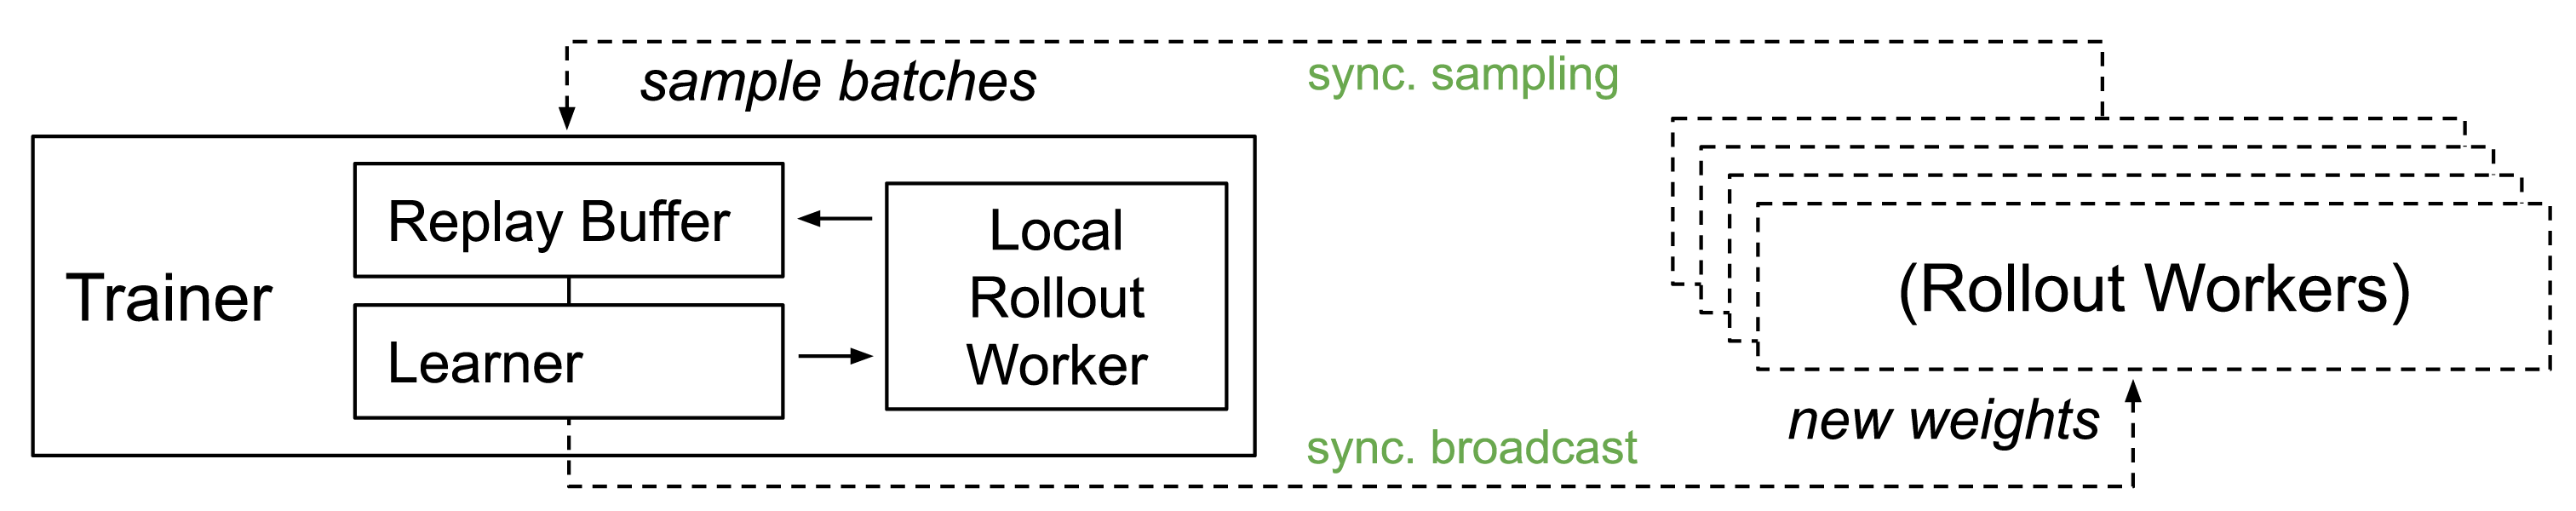
\includegraphics[scale=0.6]{gambar/rllib_dqn_architecture.png}
    % Keterangan gambar yang diinputkan
    \caption{Arsitektur DQN pada RLlib 2.0.0 \citep{rllibDocumentation}}
    % Label referensi dari gambar yang diinputkan
    \label{fig:rllib_dqn_architecture}
\end{figure}

\begin{lstlisting}[
  language=Python,
  caption={DQN-specific configs},
  label={lst:dqnSpecificConfigs}
]
self.num_atoms = 1
self.v_min = -10.0
self.v_max = 10.0
self.noisy = False
self.sigma0 = 0.5
self.dueling = True
self.hiddens = [256]
self.double_q = True
self.n_step = 1
self.before_learn_on_batch = None
self.training_intensity = None
self.td_error_loss_fn = "huber"
self.categorical_distribution_temperature = 1.0

# Changes to SimpleQConfig's default:
self.replay_buffer_config = {
    "type": "MultiAgentPrioritizedReplayBuffer",
    # Specify prioritized replay by supplying a buffer type that supports
    # prioritization, for example: MultiAgentPrioritizedReplayBuffer.
    "prioritized_replay": DEPRECATED_VALUE,
    # Size of the replay buffer. Note that if async_updates is set,
    # then each worker will have a replay buffer of this size.
    "capacity": 50000,
    "prioritized_replay_alpha": 0.6,
    # Beta parameter for sampling from prioritized replay buffer.
    "prioritized_replay_beta": 0.4,
    # Epsilon to add to the TD errors when updating priorities.
    "prioritized_replay_eps": 1e-6,
    # The number of continuous environment steps to replay at once. This may
    # be set to greater than 1 to support recurrent models.
    "replay_sequence_length": 1,
    # Whether to compute priorities on workers.
    "worker_side_prioritization": False,
}
# fmt: on
\end{lstlisting}

\subsection{Implementasi APE-X DQN}
Implementasi APE-X DQN dalam RLlib 2.0.0 menggunakan implementasi DQN yang ada dengan
tambahan \emph{distributed prioritezed experience replay} (APE-X) untuk skalabilitas
yang mencapai ratusan CPU dengan satu GPU \emph{learner}. Pada \emph{specific-configs}
yang digunakan oleh APE-X DQN, digunakan 32 \emph{rollout\_workers}. Setting \emph{rollout\_workers}
tersebut terganti oleh 3 \emph{rollout\_workers} yang dideklarasikan pada \ref{lst:customHyperparameter}.

\begin{figure}[H]
  \centering
    % Nama dari file gambar yang diinputkan
    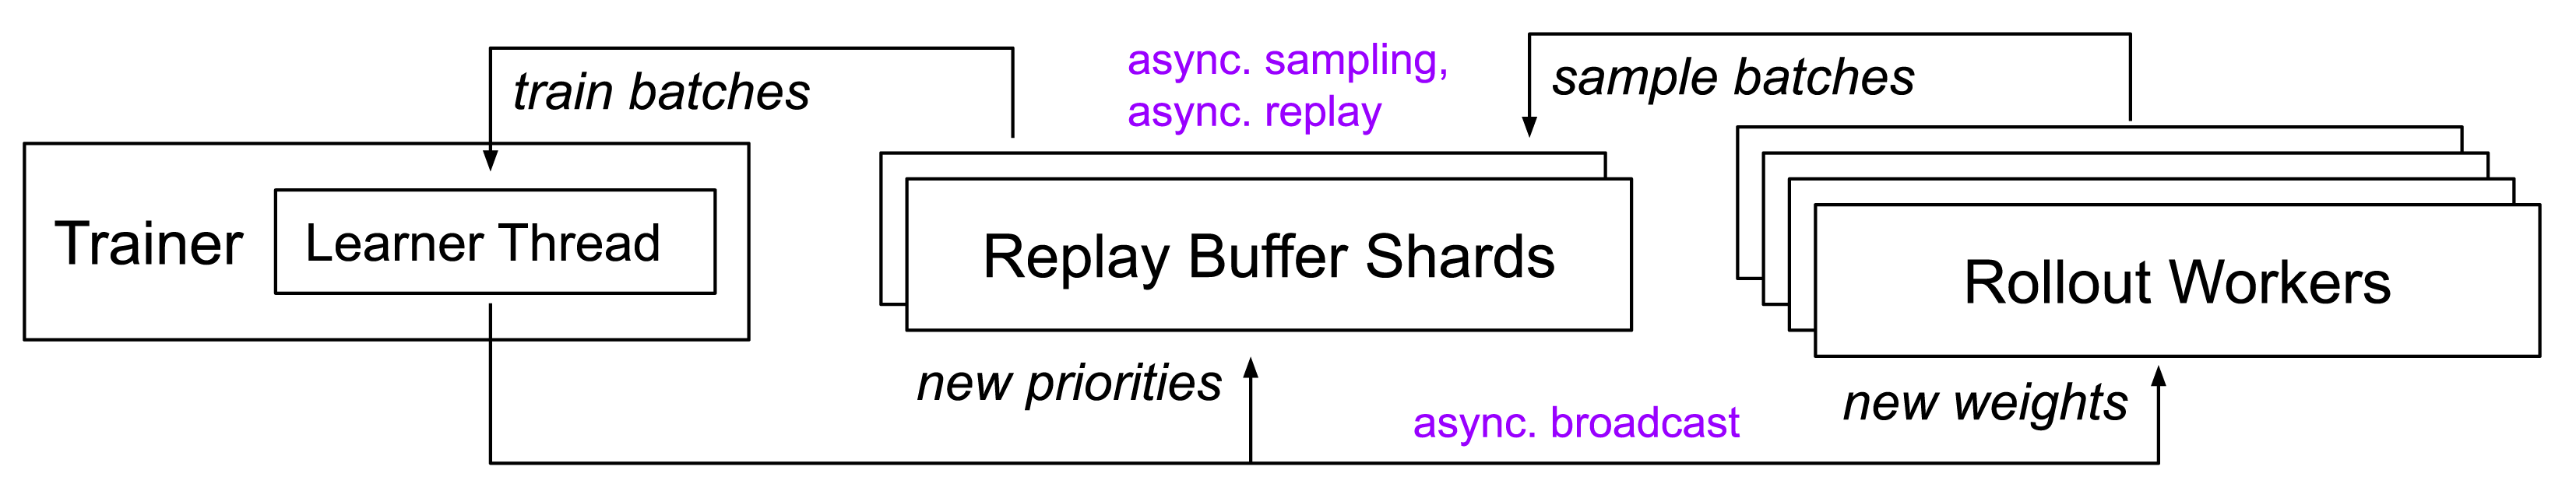
\includegraphics[scale=0.6]{gambar/rllib_apex-dqn_architecture.png}
    % Keterangan gambar yang diinputkan
    \caption{Arsitektur APE-X DQN pada RLlib 2.0.0 \citep{rllibDocumentation}}
    % Label referensi dari gambar yang diinputkan
    \label{fig:rllib_apex-dqn_architecture}
\end{figure}

\begin{lstlisting}[
  language=Python,
  caption={Cuplikan kode setting config (hyperparameter)},
  label={lst:apexDqnSpecificConfigs}
]
# APEX-DQN settings overriding DQN ones:
# .training()
self.optimizer = merge_dicts(
    DQNConfig().optimizer, {
        "max_weight_sync_delay": 400,
        "num_replay_buffer_shards": 4,
        "debug": False
    })
self.n_step = 3
self.train_batch_size = 512
self.target_network_update_freq = 500000
self.training_intensity = 1
# Number of timesteps to collect from rollout workers before we start
# sampling from replay buffers for learning. Whether we count this in agent
# steps  or environment steps depends on config["multiagent"]["count_steps_by"].
self.num_steps_sampled_before_learning_starts = 50000

# max number of inflight requests to each sampling worker
# see the AsyncRequestsManager class for more details
# Tuning these values is important when running experimens with large sample
# batches. If the sample batches are large in size, then there is the risk that
# the object store may fill up, causing the store to spill objects to disk.
# This can cause any asynchronous requests to become very slow, making your
# experiment run slowly. You can inspect the object store during your
# experiment via a call to ray memory on your headnode, and by using the ray
# dashboard. If you're seeing that the object store is filling up, turn down
# the number of remote requests in flight, or enable compression in your
# experiment of timesteps.
self.max_requests_in_flight_per_sampler_worker = 2
self.max_requests_in_flight_per_replay_worker = float("inf")
self.timeout_s_sampler_manager = 0.0
self.timeout_s_replay_manager = 0.0
# APEX-DQN is using a distributed (non local) replay buffer.
self.replay_buffer_config = {
    "no_local_replay_buffer": True,
    # Specify prioritized replay by supplying a buffer type that supports
    # prioritization
    "type": "MultiAgentPrioritizedReplayBuffer",
    "capacity": 2000000,
    # Alpha parameter for prioritized replay buffer.
    "prioritized_replay_alpha": 0.6,
    # Beta parameter for sampling from prioritized replay buffer.
    "prioritized_replay_beta": 0.4,
    # Epsilon to add to the TD errors when updating priorities.
    "prioritized_replay_eps": 1e-6,
    # Whether all shards of the replay buffer must be co-located
    # with the learner process (running the execution plan).
    # This is preferred b/c the learner process should have quick
    # access to the data from the buffer shards, avoiding network
    # traffic each time samples from the buffer(s) are drawn.
    # Set this to False for relaxing this constraint and allowing
    # replay shards to be created on node(s) other than the one
    # on which the learner is located.
    "replay_buffer_shards_colocated_with_driver": True,
    "worker_side_prioritization": True,
    # Deprecated key.
    "prioritized_replay": DEPRECATED_VALUE,
}

# .rollouts()
self.num_workers = 32
self.rollout_fragment_length = 50
self.exploration_config = {
    "type": "PerWorkerEpsilonGreedy",
}

# .resources()
self.num_gpus = 1

# .reporting()
self.min_time_s_per_iteration = 30
self.min_sample_timesteps_per_iteration = 25000

# fmt: on
\end{lstlisting}

\subsection{Implementasi PPO}
Implementasi PPO dari RLlib 2.0.0 menggunakan \emph{clipped objective} dan \emph{KL-penalty}.
Multi-GPU \emph{optimizer} RLlib meletakkan data di GPU memori untuk menghindari transfer yang tidak diperlukan
dari \emph{host memory}, sehingga performa lebih baik dari implementasi secara \emph{naive}.

\begin{figure}[H]
  \centering
    % Nama dari file gambar yang diinputkan
    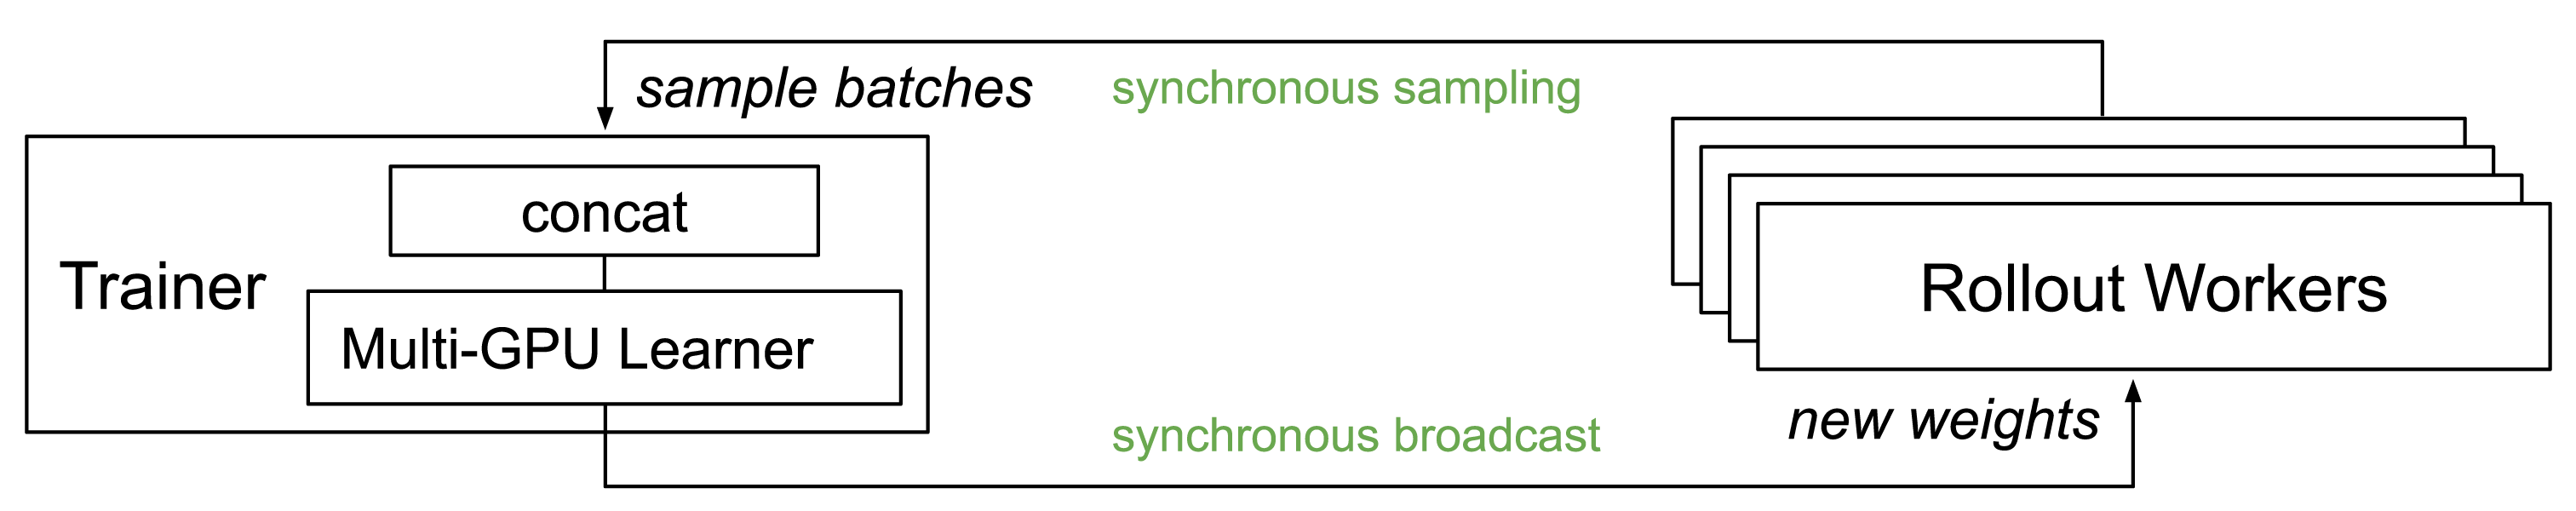
\includegraphics[scale=0.6]{gambar/rllib_ppo_architecture.png}
    % Keterangan gambar yang diinputkan
    \caption{Arsitektur PPO pada RLlib 2.0.0 \citep{rllibDocumentation}}
    % Label referensi dari gambar yang diinputkan
    \label{fig:rllib_ppo_architecture}
\end{figure}

\begin{lstlisting}[
  language=Python,
  caption={PPO-specific configs},
  label={lst:ppoSpecificConfigs}
]
# PPO specific settings:
self.lr_schedule = None
self.use_critic = True
self.use_gae = True
self.lambda_ = 1.0
self.kl_coeff = 0.2
self.sgd_minibatch_size = 128
self.num_sgd_iter = 30
self.shuffle_sequences = True
self.vf_loss_coeff = 1.0
self.entropy_coeff = 0.0
self.entropy_coeff_schedule = None
self.clip_param = 0.3
self.vf_clip_param = 10.0
self.grad_clip = None
self.kl_target = 0.01

# Override some of AlgorithmConfig's default values with PPO-specific values.
self.rollout_fragment_length = 200
self.train_batch_size = 4000
self.lr = 5e-5
self.model["vf_share_layers"] = False
    
\end{lstlisting}

\subsection{Implementasi IMPALA}
Implementasi IMPALA dari RLlib 2.0.0 menggunakan referensi kode V-trace milik DeepMind \citep{impala}.

\begin{figure}[H]
  \centering
    % Nama dari file gambar yang diinputkan
    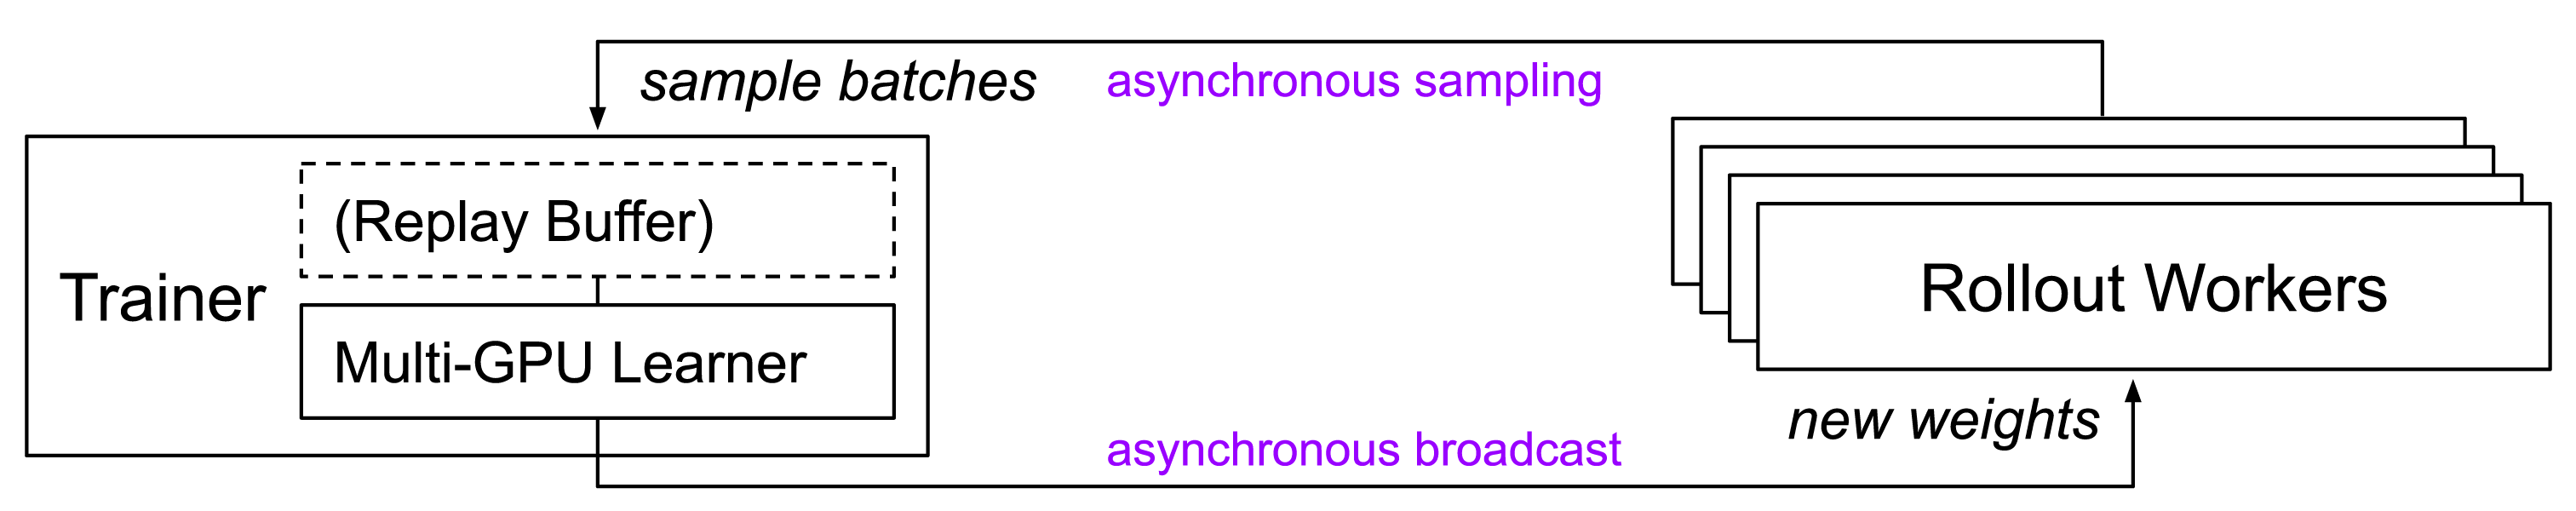
\includegraphics[scale=0.6]{gambar/rllib_impala_architecture.png}
    % Keterangan gambar yang diinputkan
    \caption{Arsitektur IMPALA pada RLlib 2.0.0 \citep{rllibDocumentation}}
    % Label referensi dari gambar yang diinputkan
    \label{fig:rllib_impala_architecture}
\end{figure}

\begin{lstlisting}[
  language=Python,
  caption={IMPALA-specific configs},
  label={lst:impalaSpecificConfigs}
]
# IMPALA specific settings:
self.vtrace = True
self.vtrace_clip_rho_threshold = 1.0
self.vtrace_clip_pg_rho_threshold = 1.0
self.vtrace_drop_last_ts = True
self.num_multi_gpu_tower_stacks = 1
self.minibatch_buffer_size = 1
self.num_sgd_iter = 1
self.replay_proportion = 0.0
self.replay_ratio = ((1 / self.replay_proportion)
                     if self.replay_proportion > 0 else 0.0)
self.replay_buffer_num_slots = 0
self.learner_queue_size = 16
self.learner_queue_timeout = 300
self.max_requests_in_flight_per_sampler_worker = 2
self.max_requests_in_flight_per_aggregator_worker = 2
self.timeout_s_sampler_manager = 0.0
self.timeout_s_aggregator_manager = 0.0
self.broadcast_interval = 1
self.num_aggregation_workers = 0
self.grad_clip = 40.0
self.opt_type = "adam"
self.lr_schedule = None
self.decay = 0.99
self.momentum = 0.0
self.epsilon = 0.1
self.vf_loss_coeff = 0.5
self.entropy_coeff = 0.01
self.entropy_coeff_schedule = None
self._separate_vf_optimizer = False
self._lr_vf = 0.0005
self.after_train_step = None

# Override some of AlgorithmConfig's default values with ARS-specific values.
self.rollout_fragment_length = 50
self.train_batch_size = 500
self.num_workers = 2
self.num_gpus = 1
self.lr = 0.0005
self.min_time_s_per_iteration = 10
    
\end{lstlisting}